% *** Authors should verify (and, if needed, correct) their LaTeX system  ***
% *** with the testflow diagnostic prior to trusting their LaTeX platform ***
% *** with production work. IEEE's font choices can trigger bugs that do  ***
% *** not appear when using other class files.                            ***
% The testflow support page is at:
% http://www.michaelshell.org/tex/testflow/


%%*************************************************************************
%% Legal Notice:
%% This code is offered as-is without any warranty either expressed or
%% implied; without even the implied warranty of MERCHANTABILITY or
%% FITNESS FOR A PARTICULAR PURPOSE!
%% User assumes all risk.
%% In no event shall IEEE or any contributor to this code be liable for
%% any damages or losses, including, but not limited to, incidental,
%% consequential, or any other damages, resulting from the use or misuse
%% of any information contained here.
%%
%% All comments are the opinions of their respective authors and are not
%% necessarily endorsed by the IEEE.
%%
%% This work is distributed under the LaTeX Project Public License (LPPL)
%% ( http://www.latex-project.org/ ) version 1.3, and may be freely used,
%% distributed and modified. A copy of the LPPL, version 1.3, is included
%% in the base LaTeX documentation of all distributions of LaTeX released
%% 2003/12/01 or later.
%% Retain all contribution notices and credits.
%% ** Modified files should be clearly indicated as such, including  **
%% ** renaming them and changing author support contact information. **
%%
%% File list of work: IEEEtran.cls, New_IEEEtran_how-to.pdf, bare_jrnl_new_sample4.tex,
%%*************************************************************************
\PassOptionsToPackage{unicode}{hyperref}
\PassOptionsToPackage{hyphens}{url}
\PassOptionsToPackage{dvipsnames,svgnames,x11names}{xcolor}
% Note that the a4paper option is mainly intended so that authors in
% countries using A4 can easily print to A4 and see how their papers will
% look in print - the typesetting of the document will not typically be
% affected with changes in paper size (but the bottom and side margins will).
% Use the testflow package mentioned above to verify correct handling of
% both paper sizes by the user's LaTeX system.
%
% Also note that the "draftcls" or "draftclsnofoot", not "draft", option
% should be used if it is desired that the figures are to be displayed in
% draft mode.
%
\documentclass[
  journal,
]{IEEEtran}%
% If IEEEtran.cls has not been installed into the LaTeX system files,
% manually specify the path to it like:
% \documentclass[journal]{../sty/IEEEtran}
\usepackage[cmex10]{amsmath}
\usepackage{amssymb}
\usepackage{iftex}
\ifPDFTeX
  \usepackage[T1]{fontenc}
  \usepackage[utf8]{inputenc}
  \usepackage{textcomp} % provide euro and other symbols
\else % if luatex or xetex
  \usepackage{unicode-math} % this also loads fontspec
  \defaultfontfeatures{Scale=MatchLowercase}
  \defaultfontfeatures[\rmfamily]{Ligatures=TeX,Scale=1}
\fi
%\usepackage{lmodern}
\ifPDFTeX\else
\fi
% Use upquote if available, for straight quotes in verbatim environments
\IfFileExists{upquote.sty}{\usepackage{upquote}}{}
\IfFileExists{microtype.sty}{% use microtype if available
  \usepackage[]{microtype}
  \UseMicrotypeSet[protrusion]{basicmath} % disable protrusion for tt fonts
}{}
\makeatletter
\parindent    1.0em
\ifCLASSOPTIONcompsoc
  \parindent    1.5em
\fi
\makeatother
\usepackage{xcolor}
\setlength{\emergencystretch}{3em} % prevent overfull lines

\setcounter{secnumdepth}{5}
% Make \paragraph and \subparagraph free-standing
\ifx\paragraph\undefined\else
  \let\oldparagraph\paragraph
  \renewcommand{\paragraph}[1]{\oldparagraph{#1}\mbox{}}
\fi
\ifx\subparagraph\undefined\else
  \let\oldsubparagraph\subparagraph
  \renewcommand{\subparagraph}[1]{\oldsubparagraph{#1}\mbox{}}
\fi

\usepackage{longtable,booktabs,array}
\newcounter{none} % for unnumbered tables
\usepackage{calc} % for calculating minipage widths
% Correct order of tables after \paragraph or \subparagraph
\usepackage{etoolbox}
\makeatletter
\patchcmd\longtable{\par}{\if@noskipsec\mbox{}\fi\par}{}{}
\makeatother
% Allow footnotes in longtable head/foot
\IfFileExists{footnotehyper.sty}{\usepackage{footnotehyper}}{\usepackage{footnote}}
\makesavenoteenv{longtable}
\usepackage{graphicx}
\makeatletter
\newsavebox\pandoc@box
\newcommand*\pandocbounded[1]{% scales image to fit in text height/width
  \sbox\pandoc@box{#1}%
  \Gscale@div\@tempa{\textheight}{\dimexpr\ht\pandoc@box+\dp\pandoc@box\relax}%
  \Gscale@div\@tempb{\linewidth}{\wd\pandoc@box}%
  \ifdim\@tempb\p@<\@tempa\p@\let\@tempa\@tempb\fi% select the smaller of both
  \ifdim\@tempa\p@<\p@\scalebox{\@tempa}{\usebox\pandoc@box}%
  \else\usebox{\pandoc@box}%
  \fi%
}
% Set default figure placement to htbp
\def\fps@figure{htbp}
\makeatother





\setlength{\emergencystretch}{3em} % prevent overfull lines

\providecommand{\tightlist}{%
  \setlength{\itemsep}{0pt}\setlength{\parskip}{0pt}}



 


\usepackage{physics}
\usepackage[version=3]{mhchem}
\usepackage{orcidlink}
\usepackage{float}
\floatplacement{table}{htb}
\makeatletter
\@ifpackageloaded{caption}{}{\usepackage{caption}}
\AtBeginDocument{%
\ifdefined\contentsname
  \renewcommand*\contentsname{Table of contents}
\else
  \newcommand\contentsname{Table of contents}
\fi
\ifdefined\listfigurename
  \renewcommand*\listfigurename{List of Figures}
\else
  \newcommand\listfigurename{List of Figures}
\fi
\ifdefined\listtablename
  \renewcommand*\listtablename{List of Tables}
\else
  \newcommand\listtablename{List of Tables}
\fi
\ifdefined\figurename
  \renewcommand*\figurename{Fig.}
\else
  \newcommand\figurename{Fig.}
\fi
\ifdefined\tablename
  \renewcommand*\tablename{Table}
\else
  \newcommand\tablename{Table}
\fi
}
\@ifpackageloaded{float}{}{\usepackage{float}}
\floatstyle{ruled}
\@ifundefined{c@chapter}{\newfloat{codelisting}{h}{lop}}{\newfloat{codelisting}{h}{lop}[chapter]}
\floatname{codelisting}{Listing}
\newcommand*\listoflistings{\listof{codelisting}{List of Listings}}
\makeatother
\makeatletter
\makeatother
\makeatletter
\@ifpackageloaded{caption}{}{\usepackage{caption}}
\@ifpackageloaded{subcaption}{}{\usepackage{subcaption}}
\makeatother
\usepackage[skip=2pt,font=footnotesize]{caption}
%\captionsetup{format=myformat}
\ifLuaTeX
  \usepackage{selnolig}  % disable illegal ligatures
\fi
\IfFileExists{bookmark.sty}{\usepackage{bookmark}}{\usepackage{hyperref}}
\IfFileExists{xurl.sty}{\usepackage{xurl}}{} % add URL line breaks if available
\urlstyle{same} % disable monospaced font for URLs
\hypersetup{
  pdftitle={A Sample Article Using quarto-ieee for IEEE Journal and Transactions},
  pdfauthor={David Folio; John Doe},
  pdfkeywords={IEEE, IEEEtran, journal, Quarto, Pandoc, template},
  colorlinks=true,
  linkcolor={blue},
  filecolor={Maroon},
  citecolor={Blue},
  urlcolor={Blue},
  pdfcreator={LaTeX via pandoc}}

% *** Do not adjust lengths that control margins, column widths, etc. ***
% *** Do not use packages that alter fonts (such as pslatex).         ***
% There should be no need to do such things with IEEEtran.cls V1.6 and later.
% (Unless specifically asked to do so by the journal or conference you plan
% to submit to, of course. )


% correct bad hyphenation here
\hyphenation{op-tical net-works semi-conduc-tor}

%
% paper title
% can use linebreaks \\ within to get better formatting as desired
% Do not put math or special symbols in the title.
% paper title
% can use linebreaks \\ within to get better formatting as desired
% Do not put math or special symbols in the title.
\title{A Sample Article Using \texttt{quarto-ieee} for IEEE Journal and
Transactions}

\author{
\thanks{The \texttt{quarto-ieee} template is freely available under the
MIT license on github: \url{https://github.com/dfolio/quarto-ieee}.}
David Folio\orcidlink{0000-0001-9430-6091},~\IEEEmembership{Member,
IEEE}
and~John Doe%
\thanks{David Folio is with Laboratoire Prisme, INSA Centre Val de
Loire, Bourges, 18800 France%
  Corresponding author: david.folio@insa-cvl.fr
}
\thanks{Unknown affiliation}
%by-author.affiliations
\thanks{John Doe is with Anonymous University%
}
%by-author.affiliations
\thanks{Template created June 23, 2023; revised
\texttt{r\ format(Sys.Date(),format=\textquotesingle{}\%B\ \%d,\ \%Y\textquotesingle{})}.}
}
\begin{document}

% The paper headers
\markboth{Journal XXX, Month Year}{D. Folio: A Sample Article Using
quarto-ieee}

% use for special paper notices

% make the title area
\maketitle

% As a general rule, do not put math, special symbols or citations
% in the abstract or keywords.
\begin{abstract}
This document describes the most common article elements and how to use
the \texttt{quarto-ieee} class with Pandoc/Quarto-Markdown to produce
files that are suitable for submission to IEEE journals.\\
\texttt{quarto-ieee} can produce conference, journal, and technical note
(correspondence) papers with a suitable choice of class options. It
intends to generate PDF and HTML outputs that closely mimick what IEEE
would generate.
\end{abstract}
% Note that keywords are not normally used for peerreview papers.
\begin{IEEEkeywords}
IEEE, IEEEtran, journal, Quarto, Pandoc, template
\end{IEEEkeywords}

% For peer review papers, you can put extra information on the cover
% page as needed:
% \ifCLASSOPTIONpeerreview
% \begin{center} \bfseries EDICS Category: 3-BBND \end{center}
% \fi
%
% For peerreview papers, this IEEEtran command inserts a page break and
% creates the second title. It will be ignored for other modes.
% \IEEEpeerreviewmaketitle


\section{I. Introduction}\label{i.-introduction}

Population aging is reshaping healthcare, labor, family structures, and
public services. In response, digital systems for older adults have
grown rapidly, especially in telehealth, remote monitoring, medication
support, and care coordination. These systems are valuable, but many are
built around narrow assumptions: that old age is primarily a condition
of decline, risk, and dependency.

That assumption is socially and technically limiting. Older adults are
not only patients or service users. They are also storytellers, mentors,
workers, caregivers, citizens, spiritual beings, and bearers of memory
and legacy. Their wellbeing depends not only on safety and functional
support, but also on continuity of identity, meaningful relationships,
opportunities to contribute, and the capacity to interpret life events
within a coherent story.

This paper proposes GRACE---Growing, Resourceful, Active, and Enriched
Life---as a socio-technical ecosystem for elder wellbeing. GRACE is an
intelligent community computing framework organized around five
relational domains: 1) spiritual self, 2) family and friends, 3) working
colleagues, 4) communities, and 5) the wider world, including markets
and public services. GRACE is grounded in the premise that elder
wellbeing is relational and that the quality of relationships shapes the
exchange of care, recognition, participation, and contribution.

The central design claim of GRACE is that narrative identity should be
treated as a core systems concept. Older adults should not be modeled
merely through static profiles, health states, or risk scores. They
should be understood as persons living through unfolding stories. GRACE
therefore acts as a live autobiographical ecosystem, helping elders
remain connected to selfhood across daily life, transitions, and
adversity. A high-level overview is shown in Fig. 1, with the multiagent
architecture shown in Fig. 2 and the dynamic closed-loop logic in Fig.
3.

To operationalize this vision, the paper introduces the GRACE Index, a
daily measure of whether a person remains ``in the zone'' of narrative
selfhood. The paper further adds three innovations: 1) a Daily Story
Creation Engine that frames lived experience through the hero's journey,
2) an AI-based Fast State Predictor that forecasts near-future wellbeing
state, and 3) a Smart Stimulus Agent that initiates timely, personalized
prompts to preserve wellbeing and authorship. Finally, the paper
proposes an agent-based simulation design to demonstrate these
innovations.

\subsection{Contributions}\label{contributions}

\begin{enumerate}
\def\labelenumi{\arabic{enumi}.}
\tightlist
\item
  A socio-technical framework for elder wellbeing centered on narrative
  identity, relationship quality, and contribution exchange.
\item
  The GRACE Index, a daily metric of narrative selfhood and adaptive
  continuity.
\item
  Three AI-enabled innovations---daily story creation, fast state
  prediction, and smart stimuli---for anticipatory wellbeing support.
\item
  An agent-based simulation design for evaluating these mechanisms
  before real-world deployment.
\end{enumerate}

\section{II. Related Work}\label{ii.-related-work}

\subsection{A. Aging Technologies and Deficit-Oriented
Design}\label{a.-aging-technologies-and-deficit-oriented-design}

Technologies for older adults have often focused on safety,
surveillance, and functional support (Sixsmith \& Gutman, 2013; Czaja et
al., 2006; Mitzner et al., 2010). While these systems can improve
independence and care delivery, they may also reproduce deficit-oriented
assumptions about aging. HCI scholarship has argued that such framings
narrow the design space and underplay agency, participation, and dignity
(Vines et al., 2015).

\subsection{B. Social Connectedness and
Wellbeing}\label{b.-social-connectedness-and-wellbeing}

Social relationships are strongly associated with wellbeing, resilience,
and mortality outcomes (Holt-Lunstad et al., 2010). Social isolation and
perceived loneliness can negatively affect cognition and health
(Cacioppo \& Hawkley, 2009). In later life, relationship quality matters
as much as contact frequency, including dimensions such as reciprocity,
belonging, and social integration (Cornwell \& Waite, 2009; Berkman et
al., 2000).

\subsection{C. Narrative Identity and Later
Life}\label{c.-narrative-identity-and-later-life}

Narrative identity theory suggests that individuals construct a sense of
self through evolving life stories (McAdams, 2001; Habermas \& Bluck,
2000; Singer, 2004). In later life, autobiographical continuity and life
review become especially important for meaning-making, legacy, and
coping with transition (Butler, 1963; Bohlmeijer et al., 2007). Yet most
digital systems do not operationalize narrative identity as a core
computational construct.

\subsection{D. Generativity and Productive
Aging}\label{d.-generativity-and-productive-aging}

Older adults continue to contribute through mentoring, caregiving,
volunteering, advising, and cultural transmission. Generativity is a
major source of meaning and self-worth (McAdams \& de St.~Aubin, 1992;
Erikson, 1982). Productive aging research likewise emphasizes the value
of creating roles and systems that support continued contribution
(Morrow-Howell et al., 2017).

\subsection{E. Community Computing, Multiagent Systems, and
Human-Centered
AI}\label{e.-community-computing-multiagent-systems-and-human-centered-ai}

Community informatics has shown how digital infrastructures can support
participation, local engagement, and social inclusion (Gurstein, 2007;
Carroll, 2014). Multiagent systems offer a framework for distributed
intelligence, coordination, and adaptive decision-making (Jennings et
al., 1998; Wooldridge, 2009). Human-centered AI emphasizes reliability,
safety, and alignment with human values (Shneiderman, 2020). GRACE
integrates these strands into a single socio-technical architecture.

\subsection{F. Research Gap}\label{f.-research-gap}

Existing work rarely integrates all of the following in one coherent
framework: narrative identity, relationship quality, contribution
exchange, community participation, institutional and market access,
predictive wellbeing support. GRACE addresses this gap by proposing a
narrative-centered, socially grounded AI ecosystem for elder wellbeing.

\section{III. GRACE as a Socio-Technical
Ecosystem}\label{iii.-grace-as-a-socio-technical-ecosystem}

The overall socio-technical structure of GRACE is illustrated in Fig. 1.
The five relational domains, their functions, and example system
supports are summarized in Table I.

\subsection{A. Core Premise}\label{a.-core-premise}

GRACE is based on a simple claim: elder wellbeing emerges from the
interaction of identity, relationships, contribution, and access. A
person flourishes when they remain connected to who they are, to people
who matter, to ways of contributing, and to the broader systems that
structure everyday life.

\subsection{B. Five Relational
Domains}\label{b.-five-relational-domains}

GRACE supports the elder's relationship with: 1. Spiritual self 2.
Family and friends 3. Working colleagues 4. Communities 5. Wider world,
including markets and public services.

{\def\LTcaptype{none} % do not increment counter
\begin{longtable}[]{@{}
  >{\raggedright\arraybackslash}p{(\linewidth - 6\tabcolsep) * \real{0.2500}}
  >{\raggedright\arraybackslash}p{(\linewidth - 6\tabcolsep) * \real{0.2500}}
  >{\raggedright\arraybackslash}p{(\linewidth - 6\tabcolsep) * \real{0.2500}}
  >{\raggedright\arraybackslash}p{(\linewidth - 6\tabcolsep) * \real{0.2500}}@{}}
\toprule\noalign{}
\begin{minipage}[b]{\linewidth}\raggedright
Domain
\end{minipage} & \begin{minipage}[b]{\linewidth}\raggedright
Description
\end{minipage} & \begin{minipage}[b]{\linewidth}\raggedright
Wellbeing Functions
\end{minipage} & \begin{minipage}[b]{\linewidth}\raggedright
Example System Supports
\end{minipage} \\
\midrule\noalign{}
\endhead
\bottomrule\noalign{}
\endlastfoot
Spiritual Self & Inner life, values, faith, reflection, existential
orientation & peace, meaning, hope, acceptance, moral continuity &
reflection prompts, prayer/meditation support, ritual reminders,
grief-sensitive dialogue \\
Family and Friends & Intimate and enduring personal relationships &
belonging, affection, care continuity, emotional security, shared memory
& family coordination, message prompts, memory sharing, visit
planning \\
Working Colleagues & Ongoing or legacy vocational and professional ties
& role continuity, usefulness, recognition, mentoring, productive
identity & mentoring matching, advisory opportunities, skill-sharing,
encore work prompts \\
Communities & Local groups, associations, faith communities,
neighborhoods, civic groups & participation, recognition, mutual aid,
collective belonging & event discovery, volunteering prompts, group
participation support, community connectors \\
Wider World & Markets, institutions, services, transport, civic systems,
public services & inclusion, access, autonomy, service reach, economic
and civic participation & service navigation, benefits support,
transport coordination, marketplace access \\
\end{longtable}
}

\subsection{C. Narrative Identity as System
Core}\label{c.-narrative-identity-as-system-core}

Rather than using a conventional user profile, GRACE maintains a Living
Autobiography Model. Its principal constructs are summarized in Table
II.

{\def\LTcaptype{none} % do not increment counter
\begin{longtable}[]{@{}
  >{\raggedright\arraybackslash}p{(\linewidth - 6\tabcolsep) * \real{0.2500}}
  >{\raggedright\arraybackslash}p{(\linewidth - 6\tabcolsep) * \real{0.2500}}
  >{\raggedright\arraybackslash}p{(\linewidth - 6\tabcolsep) * \real{0.2500}}
  >{\raggedright\arraybackslash}p{(\linewidth - 6\tabcolsep) * \real{0.2500}}@{}}
\toprule\noalign{}
\begin{minipage}[b]{\linewidth}\raggedright
Construct
\end{minipage} & \begin{minipage}[b]{\linewidth}\raggedright
Description
\end{minipage} & \begin{minipage}[b]{\linewidth}\raggedright
Examples
\end{minipage} & \begin{minipage}[b]{\linewidth}\raggedright
Function
\end{minipage} \\
\midrule\noalign{}
\endhead
\bottomrule\noalign{}
\endlastfoot
Life Chapters & Major periods or phases of life & childhood, career
phase, retirement, caregiving years & supports contextual interpretation
of current events \\
Major Transitions & Turning points and disruptions & bereavement,
migration, illness onset, retirement & supports sensitivity to recurring
vulnerabilities and resilience patterns \\
Key Relationships & Important persons and social ties & spouse,
children, friends, mentor, colleague & informs relational prompts and
support priorities \\
Roles and Identities & Enduring self-definitions & parent, teacher,
engineer, volunteer, believer & supports role continuity and
contribution opportunities \\
Values and Beliefs & Moral, spiritual, and existential commitments &
faith, service, independence, compassion & aligns prompts and
interventions with personal meaning \\
Strengths and Skills & Capabilities and resources & mentoring,
storytelling, teaching, organizing & supports contribution matching \\
Meaningful Places & Places of emotional or narrative significance &
family home, workplace, temple, neighborhood park & supports memory
prompts and place-based engagement \\
Rituals and Traditions & Recurrent meaningful practices & weekly
worship, family dinners, anniversaries & supports temporal and spiritual
grounding \\
Significant Memories & Events with autobiographical weight & marriage,
awards, losses, milestones & supports story creation and identity
continuity \\
Present Concerns & Current needs and stresses & loneliness, mobility
limits, family conflict & supports adaptive intervention \\
Future Hopes & Forward-looking aims & legacy project, reconnecting with
family, community service & supports future-oriented narrative
continuity \\
\end{longtable}
}

\subsection{D. Theater-of-Life
Perspective}\label{d.-theater-of-life-perspective}

GRACE may be understood as a theater of life: the elder is the lead
performer and author, life settings are stages, daily events are scenes,
human and AI participants form the cast, and narrative identity is the
script in progress. This metaphor is not decorative; it is a design
principle. It emphasizes authorship, visibility, and continuity.


% Can use something like this to put references on a page
% by themselves when using endfloat and the captionsoff option.
\ifCLASSOPTIONcaptionsoff
  \newpage
\fi

% trigger a \newpage just before the given reference
% number - used to balance the columns on the last page
% adjust value as needed - may need to be readjusted if
% the document is modified later
%\IEEEtriggeratref{8}
% The "triggered" command can be changed if desired:
%\IEEEtriggercmd{\enlargethispage{-5in}}

% Uncomment when use biblatex with style=ieee
%\renewcommand{\bibfont}{\footnotesize} % for IEEE bibfont size

\pagebreak[3]
\begin{IEEEbiography}[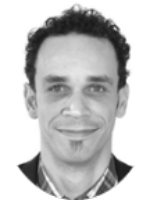
\includegraphics{david-folio.png}]{David Folio}
Use \texttt{IEEEbiography} with figure as option and the author name as
the argument followed by the biography text.
\end{IEEEbiography}
\begin{IEEEbiographynophoto}{John Doe}
Use \texttt{IEEEbiographynophoto} and the author name as the argument
followed by the biography text.
\end{IEEEbiographynophoto}
% that's all folks
\end{document}

